\documentclass[11pt]{article}

\usepackage{filecontents}
\begin{filecontents}{\jobname.bib}
@article{hohna2014probabilistic,
  title={Probabilistic graphical model representation in phylogenetics},
  author={H{\"o}hna, Sebastian and Heath, Tracy A and Boussau, Bastien and Landis, Michael J and Ronquist, Fredrik and Huelsenbeck, John P},
  journal={Systematic biology},
  volume={63},
  number={5},
  pages={753--771},
  year={2014},
  publisher={Oxford University Press}
}
@article{leliaert2014dna,
  title={DNA-based species delimitation in algae},
  author={Leliaert, Frederik and Verbruggen, Heroen and Vanormelingen, Pieter and Steen, Frederique and L{\'o}pez-Bautista, Juan M and Zuccarello, Giuseppe C and De Clerck, Olivier},
  journal={European journal of phycology},
  volume={49},
  number={2},
  pages={179--196},
  year={2014},
  publisher={Taylor \& Francis}
}
\end{filecontents}

\usepackage{natbib}
\usepackage{adjustbox}
\usepackage{amsmath}
\usepackage[font=footnotesize]{caption}
\usepackage[dvipsnames]{xcolor}
\usepackage{geometry}
  \geometry{margin=1in}
\usepackage{framed}
\usepackage[breaklinks]{hyperref}
\usepackage{minibox}
\usepackage[compact]{titlesec}
\usepackage{listings,color}

\definecolor{verbgray}{gray}{0.9}

\lstnewenvironment{code}{%
  \lstset{backgroundcolor=\color{verbgray},
  frame=single,
  framerule=0pt,
  basicstyle=\ttfamily\small,
  columns=fullflexible}}{}

\definecolor{shadecolor}{rgb}{.9, .9, .9}

\graphicspath{ {./figures/} }




\begin{document}


\noindent
\large
\begin{minipage}{0.5\textwidth}
\begin{flushleft} 
IB200, Spring 2016
\end{flushleft}
\end{minipage}
\begin{minipage}{0.5\textwidth}
\begin{flushright} 
\textit{University of California, Berkeley}
\end{flushright}
\end{minipage}

\vspace{0.5cm}


\begin{center}
\Large \textbf{Lab 11:} \\
Gene Tree-Species Tree Reconstruction \\ 
Using RevBayes and the Multispecies Coalescent \\
\normalsize
\textit{By Will Freyman} \\
\end{center}

\vspace{0.5cm}

\section{Before you begin}

Please download and install \textbf{RevBayes}.
RevBayes is a command line program that runs from the terminal,
please make sure you can get it running before lab.
Downloads are here: \url{http://revbayes.github.io/code.html}

Since we will be using sequence data that downloaded with RevBayes,
please run RevBayes in the RevBayes folder you downloaded it in.

The scripts used here have been modified from the excellent tutorial by Bastien Boussau and Sebastian H{\"o}hna 
posted at \url{http://revbayes.com}.

\section{Introduction to the multispecies coalescent model}

In lecture we have discussed many reasons that gene trees may differ from species trees.
These processes include horizontal tree transfer, introgression,
incomplete lineage sorting (ILS), and gene tree error.
The multispecies coalescent models ILS and deep coalescence (see Figure 1).
It does not model reticulate evolutionary processes such as introgression or hybrid speciation,
though the multispecies coalescent has been extended (with varying degrees of success) to model those processes.

There is a long history of methods that reconcile gene trees
with species trees. There are parsimony methods such as 
Minimising Deep Coalescences (MDC) that try to minimize gene duplications and losses, 
algorithmic approaches such as ASTRAL (Accurate Species TRee ALgorithm)
that are consistent with the coalescent but are not explicitly using a probabilistic method.
There are also methods that reconcile already estimated gene tree posterior distributions
such as BUCKy (Bayesian Concordance Analysis) and BEST (Bayesian Estimation of Species Trees).

However, the full probabilistic multispecies coalescent model that estimates
gene trees simultaneously with the species tree is only implemented
in a couple pieces of software. The most popular is *BEAST (starBEAST),
which is just BEAST with some extensions. It is very easy to use, but can
be a bit of a black-box if you simply rely on default priors.
Today we'll implement the multispecies coalescent in RevBayes,
and step through setting up the entire model as well as the MCMC proposals
needed to perform inference.

\subsection{Calculating coalescent probabilities}

We talked in lecture about how to calculate coalescent probabilities, but
it is important to keep in mind that two parameters of the species tree have an impact on the expected
gene tree/species tree incongruence:

\begin{enumerate}

\item \textbf{Time between speciation events:}
    As branches get shorter, the pool of alleles within the branch has less time to undergo change.
    So we can expect deep coalescence and ILS more frequently when branch lengths are short.

\item \textbf{Effective population size:}
    In large populations alleles are more likely to be carried by large numbers of individuals,
    so chance events are less likely to wipe out alleles. 
    In small populations chance events can wipe out entire alleles, resulting in less polymorphism.
    So we can expect deep coalescence and ILS more frequently when effective population sizes are large.

\end{enumerate}

\subsection{A note about ``species'' trees}

In this lab and much of the literature, we talk about gene trees nested within ``species'' trees.
Note that a species tree could more precisely be called a ``population'' tree,
and that both populations and species have fuzzy boundaries that may change depending on the
organisms and/or the scientists.
Regardless of the term you use, the important point is that the
multispecies coalescent explicitly models polymorphic lineages and ILS.

\begin{figure}
\centering
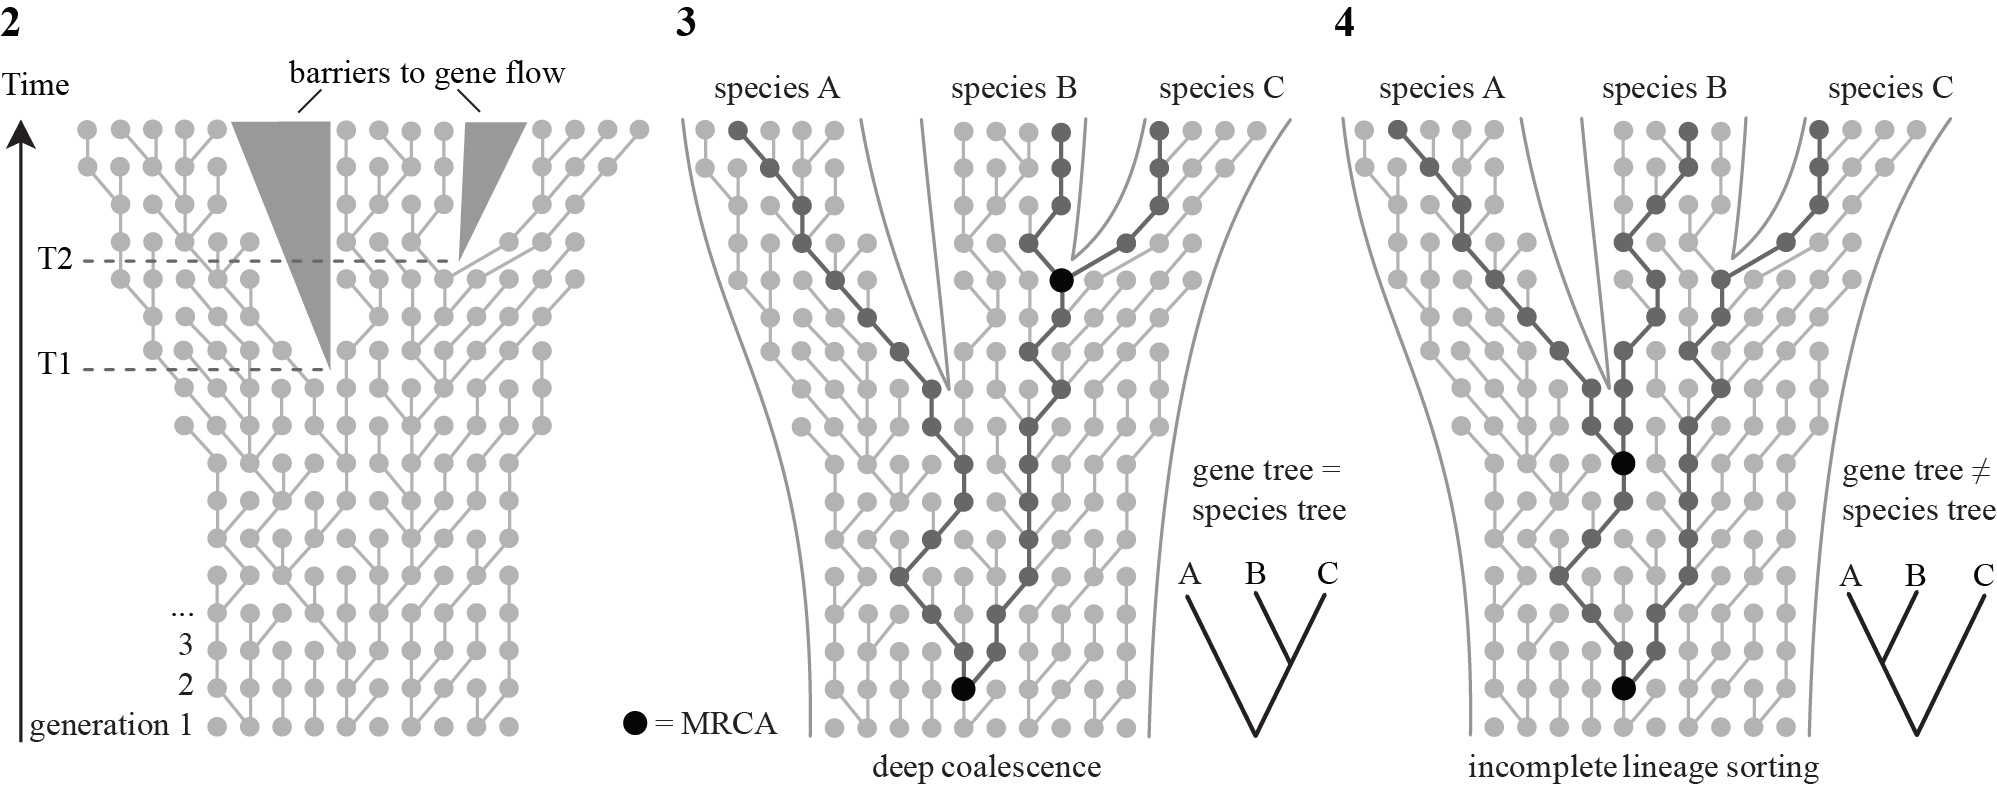
\includegraphics[width=0.9\textwidth]{ils.jpg}
\caption{
    Diagram illustrating the coalescent process and two sources of incongruence between gene-trees and species-trees:
    \textit{deep coalescence} and \textit{incomplete lineage sorting}. 
    Tree on the left: each dot represents an individual gene copy and each line connects a gene copy to its
    ancestor in the previous generation. Starting with a set of individuals in a first generation, the second generation is created by
    randomly selecting a parent from the first population; the third generation is sampled from the second, and so on. During speciation
    events (T1 and T2), where populations become separated by a barrier to gene flow, gene copies will only be sampled from within the
    same population. This coalescence process, running inside the species tree, has two important consequences. Middle tree:
    DNA divergence times may be much older than speciation times, known as \textit{deep coalescence}. As illustrated, the most recent
    common ancestor (MRCA) of two gene copy samples from species A, B and C is much older than the speciation event T1. Right tree:
    deep coalescence in combination with incomplete fixation of gene lineages within species lineages (\textit{incomplete lineage sorting}) may
    result in a gene tree and species tree with different topologies. For example, the gene tree based on three randomly sampled alleles
    would wrongly suggest a sister relationship between species A and B.
From \protect\citet{leliaert2014dna}.}
\end{figure}


\section{Implementing the multispecies coalescent in RevBayes}

Today, we'll apply the multispecies coalescent model to 10 gene alignments from 23 primate species.

\subsection{Loading our sequence data}

Start up RevBayes and load our data:
\begin{code}
locus_names = ["COIII", "FGA", "GHRmeredith", "lrpprc_169", 
               "npas3", "sim1", "tex2", "ttr", "zfy", "zic3"]

num_loci = locus_names.size()

# read in each data matrix separately
for ( i in 1:num_loci ) {
    data[i] <- readDiscreteCharacterData("data/" + locus_names[i] + ".fasta")
}

# Get some useful variables from the data. We need these later on.
n_species <- data[10].ntaxa()
taxa <- data[10].taxa()
n_branches <- 2 * n_species - 1 # number of branches in a rooted tree

# set my MCMC move index
mi = 0
\end{code}

\subsection{Species tree prior}

We'll use a constant-rate sampled-birth-death process as the prior on the species tree.
The birth-death process takes both speciation and extinction rates as its parameters.
Note, we could easily use a Yule (birth-only) prior here instead if we wanted.
We could also use rate-heterogenous birth-death processes as well.
This is the \textit{sampled} birth-death process because it requires an additional
parameter $\rho$ (or \texttt{rho}) which represents the proportion of extant lineages sampled.

First, set up the prior on speciation and extinction. There are multiple ways
to parameterize these, feel free to try variations:
\begin{code}
speciation ~ dnGamma(2,2)
relativeExtinction ~ dnBeta(1,1)
extinction := speciation * relativeExtinction
\end{code}
We can set up $\rho$ as such, because we know we sampled 23 out of the roughly 450 named primate species:
\begin{code}
sampling_fraction <- 23 / 450
\end{code}
Now we will calibrate the tree by assuming that the crown age of primates is around 75 mya. 
Our informed guess is about 75-80 mya, thus, 
we specify a normal distribution with mean 75 and standard deviation 2.5 as the prior on the root age. 
Since the root age can only be a positive real number we truncate the normal distribution at 0.
We could have additionally used fossils, but for simplicity we'll stick to just the root calibration.
\begin{code}
root ~ dnNormal(mean=75,sd=2.5,min=0.0, max=Inf)
\end{code}
Finally, we can draw our species tree (\texttt{psi} or $\psi$)
from the sampled-birth-death process:
\begin{code}
psi ~ dnBDP(lambda=speciation, mu=extinction, rootAge=root, rho=sampling_fraction, taxa=taxa)
\end{code}
Now we need to set up moves so that the MCMC can explore parameter space.
First set up moves on the diversification rates and root age:
\begin{code}
moves[++mi] = mvSlide(speciation,delta=1,tune=true,weight=2)
moves[++mi] = mvSlide(relativeExtinction,delta=1,tune=true,weight=2)
moves[++mi] = mvScale(speciation,lambda=1,tune=true,weight=2)
moves[++mi] = mvScale(relativeExtinction,lambda=1,tune=true,weight=2)
moves[++mi] = mvSlide(root,delta=1,tune=true,weight=0.2)
\end{code}
And let's add some moves for the species tree:
\begin{code}
moves[++mi] = mvNarrow(psi, weight=5.0)
moves[++mi] = mvNNI(psi, weight=1.0)
moves[++mi] = mvFNPR(psi, weight=3.0)
moves[++mi] = mvGPR(psi, weight=3.0)
moves[++mi] = mvSubtreeScale(psi, weight=3.0)
moves[++mi] = mvNodeTimeSlideUniform(psi, weight=15.0)
moves[++mi] = mvTreeNodeAgeSlide(psi, weight=100)
\end{code}

\subsection{Gene tree priors}

Now that we have set up the species tree, 
we can use the multispecies coalescent process to specify gene tree priors.
Here we will assume a constant population size for the entire tree
of 1000. This is clearly a ridiculous assumption.
\begin{code}
Ne <- 1000
\end{code}
Now we will pull each gene tree from the multispecies coalescent process prior:
\begin{code}
for (i in 1:num_loci) {

   # We need to read in files providing the link between gene names and species names
   taxon_map = readTaxonData("data/species_maps/primates_" + locus_names[i] + 
                    "_species_map.txt")

   geneTree[i] ~ dnMultiSpeciesCoalescent(speciesTree=psi, Ne=Ne, taxa=taxon_map)
}
\end{code}
Note that if \texttt{Ne} had been a vector of effective population sizes,
allowing one parameter per branch of the species tree, the same code would work.
Now we must provide MCMC proposals for the gene trees:
\begin{code}
move_species_narrow_exchange = mvSpeciesNarrow( speciesTree=psi, weight=5 )
for (i in 1:num_loci) {

   moves[++mi] = mvNNI(geneTree[i], 5.0)
   moves[++mi] = mvNarrow(geneTree[i], 5.0)
   moves[++mi] = mvFNPR(geneTree[i], 3.0)
   moves[++mi] = mvGPR(geneTree[i], 2.0)
   moves[++mi] = mvSubtreeScale(geneTree[i], 5.0)
   moves[++mi] = mvTreeScale(geneTree[i], 1.0, true, 3.0)
   moves[++mi] = mvNodeTimeSlideUniform(geneTree[i], 20.0)
   move_species_narrow_exchange.addGeneTreeVariable( geneTree[i] )

}
moves[++mi] = move_species_narrow_exchange
\end{code}

\subsection{Sequence evolution models and clock rates}

Next we need clock rates for each gene. 
These scale the branch lengths in expected number of substitutions
into time.
Here we will assume a strict clock for each gene,
however we could easily use relaxed clocks by
drawing a separate rate for each branch.
\begin{code}
for ( i in 1:num_loci ) {

   clock_rate[i] ~ dnExponential(1.0)

   moves[++mi] = mvScale(clock_rate[i], weight=1.0)
}
\end{code}
We will assign each gene the HKY+G
model of nucleotide evolution.
The HKY model takes the parameter \texttt{kappa}
which is the ratio of the transition to transversion rates,
and the parameter \texttt{pi} which
are the equilibrium frequencies for each of the four bases.
Let's set up the rate matrix \texttt{Q} for
each gene:
\begin{code}
for ( i in 1:num_loci ) {

    kappa[i] ~ dnLognormal(0,1)

    pi_prior[i] <- v(1,1,1,1)
    pi[i] ~ dnDirichlet(pi_prior[i])

    Q[i] := fnHKY(kappa[i],pi[i])

}
\end{code}
And now we'll model the gamma distributed rate variation among
sites (the +G part of the HKY+G model).
As is standard, we use a discretized gamma distribution
with four rate categories. We'll utilize an exponential
prior on the \texttt{alpha} shape parameter.
\begin{code}
for ( i in 1:num_loci ) {

    alpha_prior[i] <- 0.05
    alpha[i] ~ dnExponential( alpha_prior[i] )
    gamma_rates[i] := fnDiscretizeGamma( alpha[i], alpha[i], 4, false )

}
\end{code}
We need to add moves for 
the stationary frequencies, exchangeability rates and the shape parameter:
\begin{code}
for ( i in 1:num_loci ) {

    moves[++mi] = mvScale(kappa[i],weight=1)
    moves[++mi] = mvSimplexElementScale(pi[i],weight=2)
    moves[++mi] = mvScale(alpha[i],weight=2)

}
\end{code}
Finally, just like in last week's lab, 
we set up continuous-time Markov chain (CTMC) distributions
for sequence evolution, one for each gene.
We then clamp our sequence data to the CTMCs.
We don't set up moves for the CTMC because they
are the observed values and are therefore fixed.
\begin{code}
for ( i in 1:num_loci ) {
    
    seq[i] ~ dnPhyloCTMC(tree=geneTree[i], Q=Q[i], branchRates=clock_rate[i], 
                         siteRates=gamma_rates[i], type="DNA")
    seq[i].clamp(data[i])

}
\end{code}
And now we have completed our model.
Let's make a workspace variable to represent the model.
We can use any node of our model, here we choose to use the species tree \texttt{psi}.
\begin{code}
mymodel = model(psi)
\end{code}

\subsection{Running the MCMC analysis}

We're now ready to perform inference on our model. 
Just like before, let's set up some MCMC monitors.
\begin{code}
monitors[1] = mnScreen(printgen=10, root)
monitors[2] = mnModel(filename="output/primates_root_calibration.log", printgen=10)
monitors[3] = mnFile(filename="output/primates_root_calibration.trees", printgen=10, psi)
\end{code}
Let's additionally include monitors for each of the gene trees:
\begin{code}
for ( i in 1:num_loci ) {
    monitors[i+3] = mnFile(filename="output/primates_root_calibration_" + locus_names[i] + 
                                        ".trees", printgen=10, geneTree[i])
}
\end{code}
Here we'll perform a simple MCMC analysis. 
You could also set \texttt{nruns=2} for a replicated analysis
or use \texttt{mcmcmc} to perform Metropolis coupled MCMC with heated chains.
\begin{code}
mymcmc = mcmc(mymodel, monitors, moves)
\end{code}
And finally let's start the analysis. 
\begin{code}
mymcmc.run(generations=1000)
\end{code}
This will take about 5 minutes or so.
You may want to begin exercise 1 (below) while you wait.

\subsection{Summarizing the species tree from the posterior}

Now let's summarize the posterior distribution of species trees.
We first read in the tree trace, and then produce a \textit{maximum a posteriori} (MAP) tree.
\begin{code}
treetrace = readTreeTrace("output/primates_root_calibration.trees", treetype="clock")
mapTree(treetrace,"output/primates_root_calibration.tree")
\end{code}
Check out \texttt{primates\_root\_calibration.tree} in FigTree.

\begin{framed}
\noindent
\textbf{Exercise 1:} \\
Set up a Rev script to perform the same
analysis, except instead of using a constant
population size of 1000, estimate a population size
drawn from an exponential prior with an expected mean of 1000. 
Since the expected mean = 1/$\mu$, use \texttt{dnExponential(0.001)}.
Don't forget appropriate MCMC proposals.
\begin{enumerate}
\item Send me the Rev code you used for the population size parameter.
\item Your MCMC analysis did not converge, but look at the trace
        to get a sense of the parameter estimates. Roughly, what is
            your estimate for the population size? % around 20-30
\end{enumerate}
\end{framed}

\begin{framed}
\noindent
\textbf{Exercise 2:} \\
Set up a Rev script to to estimate
population sizes that change through time 
and across the phylogeny (one parameter for every branch).
Use whatever prior you think is appropriate.
\begin{enumerate}
\item Send me the Rev code you used for the population size parameters.
\item How does this model mix compared to the models with a constant population size? Why do you think it performed this way?
\item Concatenation is still used much more frequently than the full multispecies coalescent.
        Summarize in a sentence or two the pros and cons of using concatenation versus the multispecies coalescent.
\end{enumerate}
\end{framed}

\begin{framed}
\noindent
\textbf{Please email me the following:}
\begin{enumerate}
  \item Your MAP species tree \texttt{primates\_root\_calibration.tree}.
  \item The answers to exercises 1-2.
\end{enumerate}
\end{framed}

\bibliographystyle{plainnat}
\bibliography{\jobname} 

\end{document}

